\section{Valutazione prestazioni}
AMD Opteron (tm) Processor 6376 8 core 16 thread.

Le tempistiche indicate sono state tutte ottenute mediante le funzioni di
libreria messe a disposizione dal docente. Per ulteriori informazioni si
consulti il codice sorgente.

\begin{figure}[!ht]
  \centering
  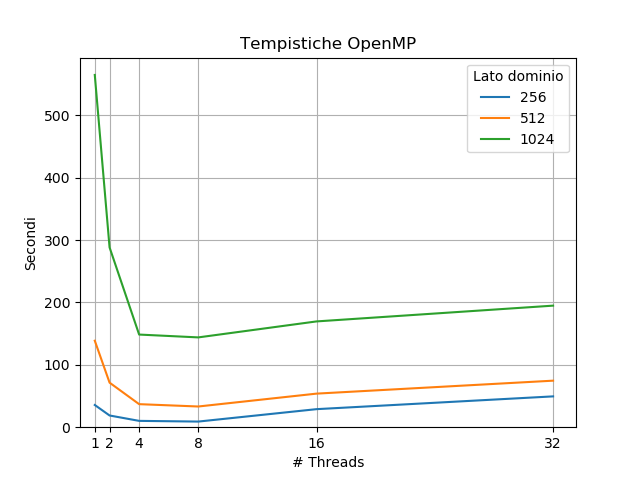
\includegraphics[scale=0.55]{./graphs/omp-timings.png}
  \caption{Comparazione tempistiche di esecuzione in OpenMP.}\label{fig:timings1}
\end{figure}

\subsection{Speedup}

Il calcolo dello speedup viene eseguito mediante la seguente formula:

\[ 
    S(p) = \frac{T_{serial}}{T_{parallel}(p)}
\]

in cui:
\begin{table}[ht]
\begin{tabular}{lll}
    p & : & \# processori/core\\
    T\textsubscript{serial}& : & tempo di esecuzione della porzione seriale
    (T\textsubscript{serial}=T\textsubscript{parallel}(1))\\
    T\textsubscript{parallel}(\textit{p}) & : & tempo di esecuzione della porzione con
    \textit{p} processori/core
\end{tabular}
\end{table}

Poiché l'implementazione della soluzione contiene porzioni di codice non
parallelizzabili (si veda la funzione \texttt{setup}), dovremmo considerare
T\textsubscript{parallel}(\textit{p}) nel seguente modo:

\[ 
T_{parallel}(p) = \alpha \cdot T_{serial} +  \frac{(1 - \alpha) \cdot
T_{serial}}{p}
\]

in cui $\alpha$ è il fattore relativo alla porzione di codice non
parallelizzabile, calcolato come segue:

\[ 
\alpha = \frac{T_{serial}}{T_{serial} + T_{parallel}}.
\]

Tuttavia, come mostrato nella seguente tabella, la porzione di codice seriale
(non parallelizzabile) impiega tempo trascurabile rispetto alla porzione di
codice parallelizzata, pertanto anche $\alpha$ assume valore trascurabile.

%\pgfmathparse{0.00140063/(0.00140063 + 14.2519)}\pgfkeys{/pgf/number format/sci}\pgfmathresult
\begin{table}[ht]
\begin{tabular}{ccccc}
\toprule
 Lato dominio & Numero passi & T\textsubscript{seriale} (\textit{s}) &
 T\textsubscript{parallelo} (\textit{s})& $\alpha$ \\
 \midrule
    256 & \multirow{2}{*}{100000} & 0.00140063 & 14.2519 & 0.00009827 \\
    1024 & & 0.02356447 & 150.2037 & 0.00015686 \\
\bottomrule
 %s_elapsed/(s_elapsed + p_elapsed)
 %0.00009827
\end{tabular}
\caption{caption}
\end{table}

Per le siffatte osservazioni, considereremo
T\textsubscript{parallel}(\textit{p}) in tal modo:

\[
T_{parallel}(p) = \frac{T_{serial}}{p}.
\]

\begin{figure}[!ht]
  \centering
  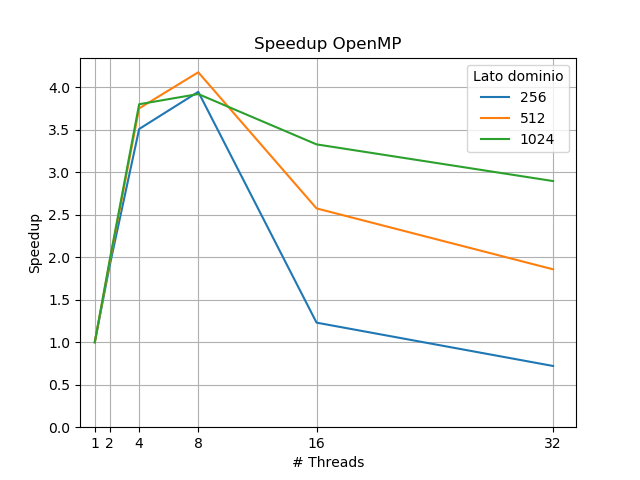
\includegraphics[scale=0.55]{./graphs/omp-speedup.png}
  \caption{Grafico dello speedup.}\label{fig:speedup1}
\end{figure}

\newpage

\subsection{Strong scaling}

\begin{figure}[!ht]
  \centering
  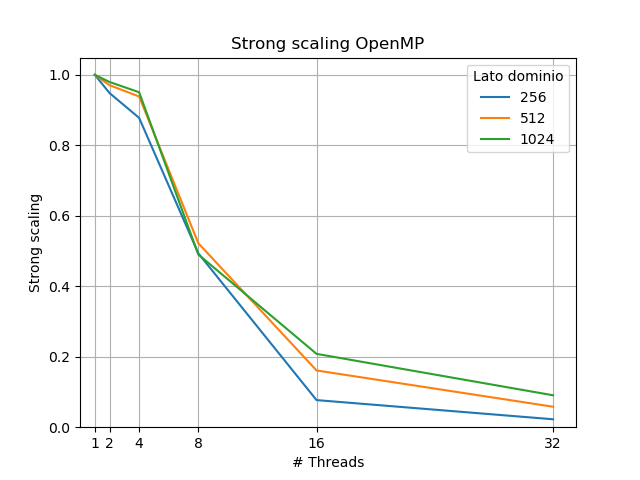
\includegraphics[scale=0.55]{./graphs/omp-strong.png}
  \caption{Grafico dello strong scaling.}\label{fig:strong1}
\end{figure}

\subsection{Weak scaling}

Dimensione del dominio:

\[
side(p) = 256 \cdot \sqrt[3]{p}
\]

come mostrato negli script di esempio del docente.

\[
W(p) = \frac{T_{1}}{T_{p}}
\]

in cui:
\begin{table}[ht]
\begin{tabular}{lll}
    p &: & \# processori/core\\
    T\textsubscript{1}&: & tempo di esecuzione di una unità di lavoro con un
    processore/core\\
    T\textsubscript{p}&: & tempo di esecuzione di \textit{p} unità di lavoro con
    \textit{p} processori/core
\end{tabular}
\end{table}

\begin{figure}[!ht]
  \centering
  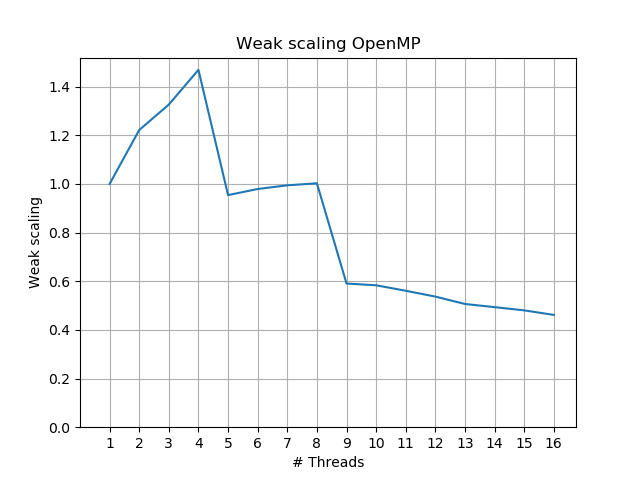
\includegraphics[scale=0.55]{./graphs/omp-weak.png}
  \caption{Grafico dello weak scaling.}\label{fig:weak1}
\end{figure}
